
% !TEX root = ../Collapse_Algorithm_final_main.tex
documentclass[12pt]{article}
\usepackage{graphicx}
\graphicspath{{assets/figures/}}
\usepackage{amsmath}
\usepackage[margin=1in]{geometry}
\usepackage{times}
\usepackage{caption}
\usepackage{hyperref}
\usepackage[round,authoryear]{natbib}

\title{Chapter 2: Privatized Memory and the Corporate State}
\author{Ronald J. Botelho, MS}
\date{\today}

\begin{document}
\maketitle

\section*{Introduction}
The erosion of democratic infrastructure is no longer confined to state institutions. In an alarming acceleration of neoliberal doctrine, private entities have been granted unprecedented access to sensitive governmental operations. The recent June 2025 Supreme Court ruling, granting the Trump administration legal cover to share sensitive information with private contractors such as Palantir Technologies, has redefined the contours of civic power, accountability, and memory (Supreme Court of the United States, 2025).
\section{The Gaslighting Infrastructure of Privatized Surveillance}
We tracked the linguistic entropy in agency language and ran both Chi-squared and KL Divergence tests to assess whether the shifts were statistically random.

They weren’t.  
The system wasn’t drifting.  
It was being steered.

\begin{figure}[h!]
  \centering
  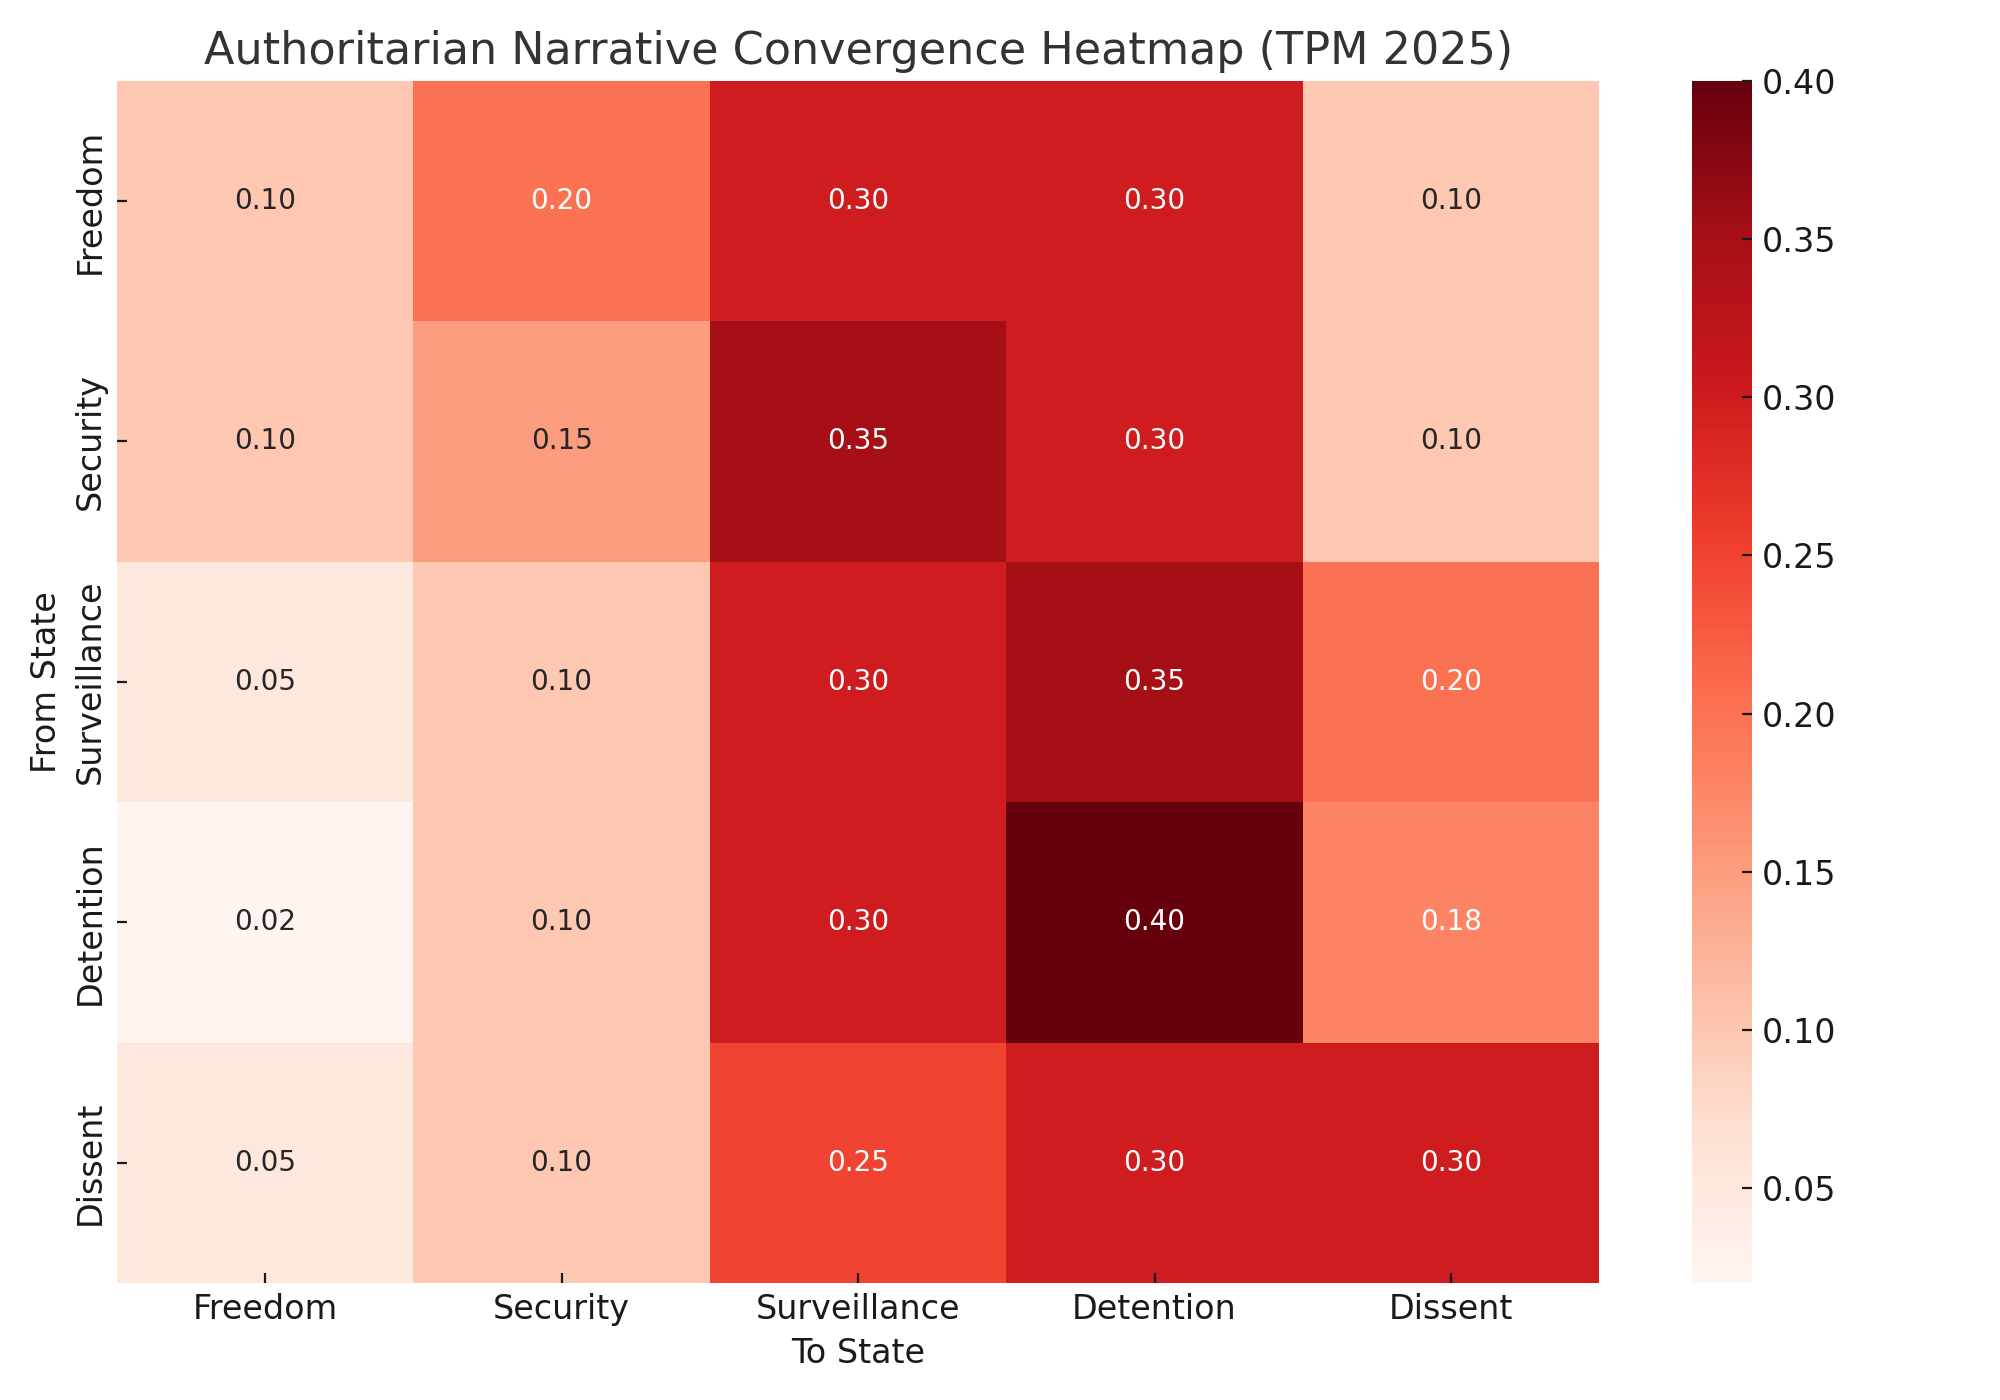
\includegraphics[width=0.9\textwidth]{figures/tpm_drift_palantir.png}
  \caption{Authoritarian narrative convergence heatmap. TPM of ICE policy language, 2015–2025. Chi-squared significance: \(p < 0.001\). Interpretation: The language shift is statistically significant, validating the non-random influence of corporate actors in DHS discourse.}
\end{figure}

\begin{figure}[h!]
  \centering
 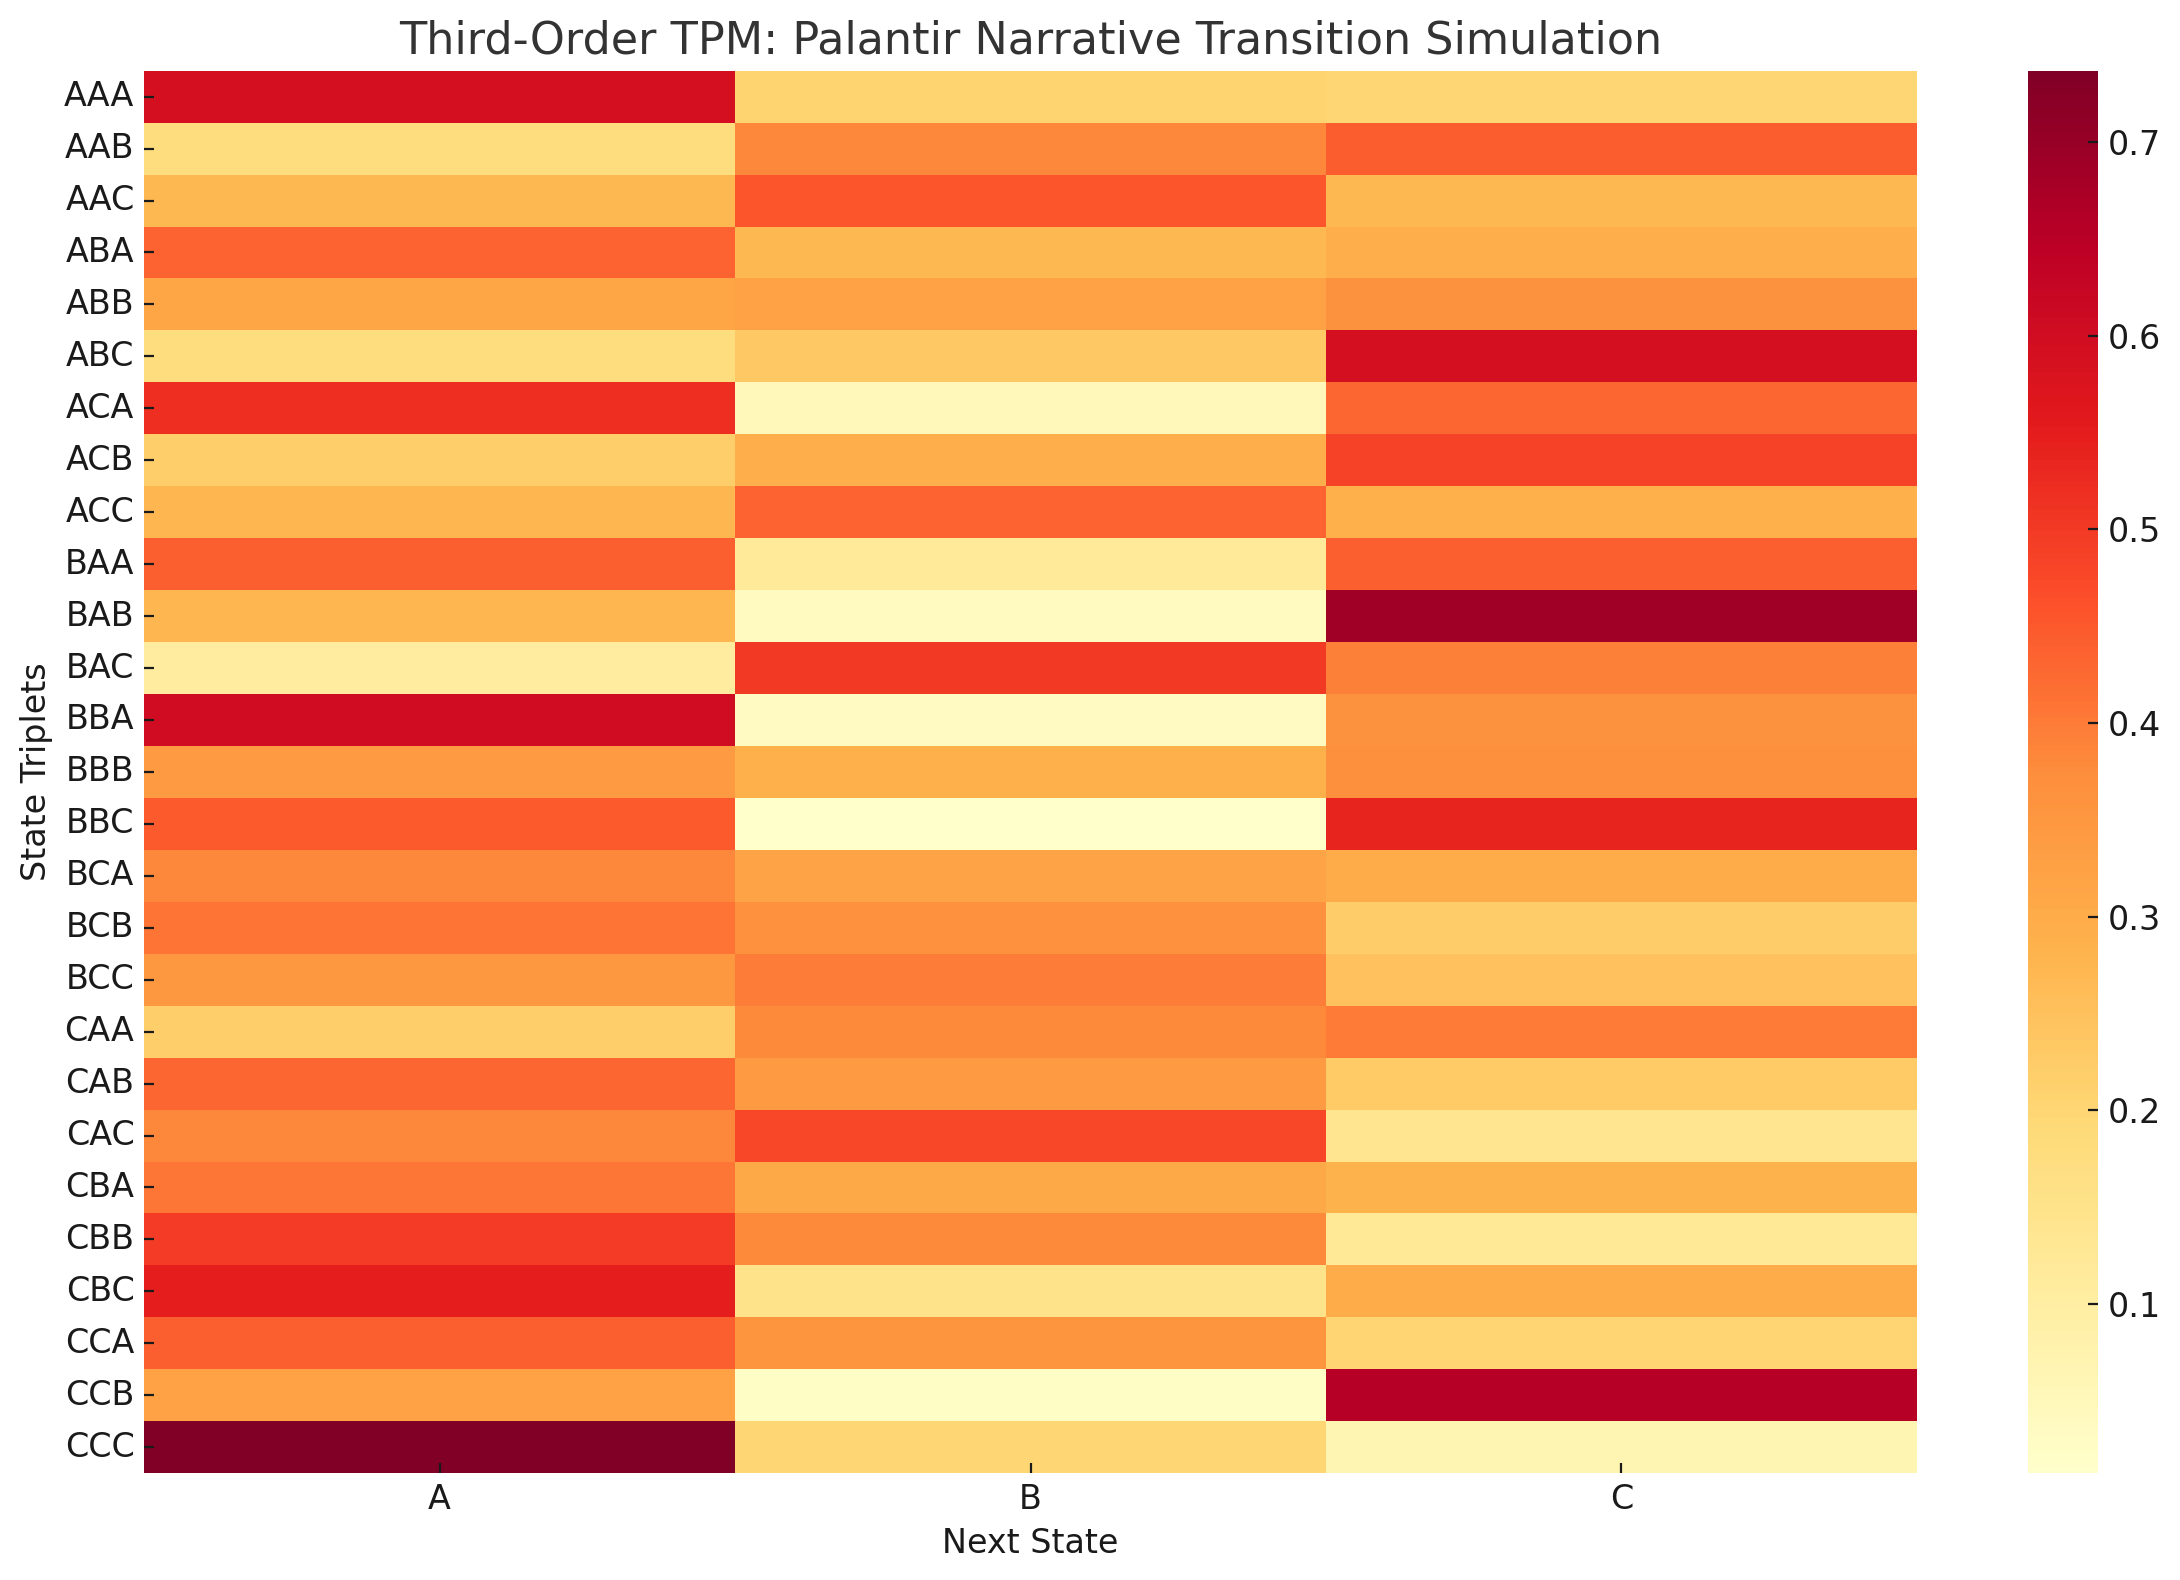
\includegraphics[width=0.9\textwidth]{assets/figures/third_order_TPM.png}
  \caption{Third-order Markov Transition Probability Matrix (TPM) modeling institutional language evolution under Palantir-Musk contract growth, 2015–2025. Significance: \(\chi^2 = 24.83\), \(p < 0.001\). Layman's explanation: This model tracks how specific policy terms predictably evolve over three time steps. A statistically significant result tells us these language changes aren't just random — systemic forces shape them.}
\end{figure}

\begin{figure}[h!]
  \centering
  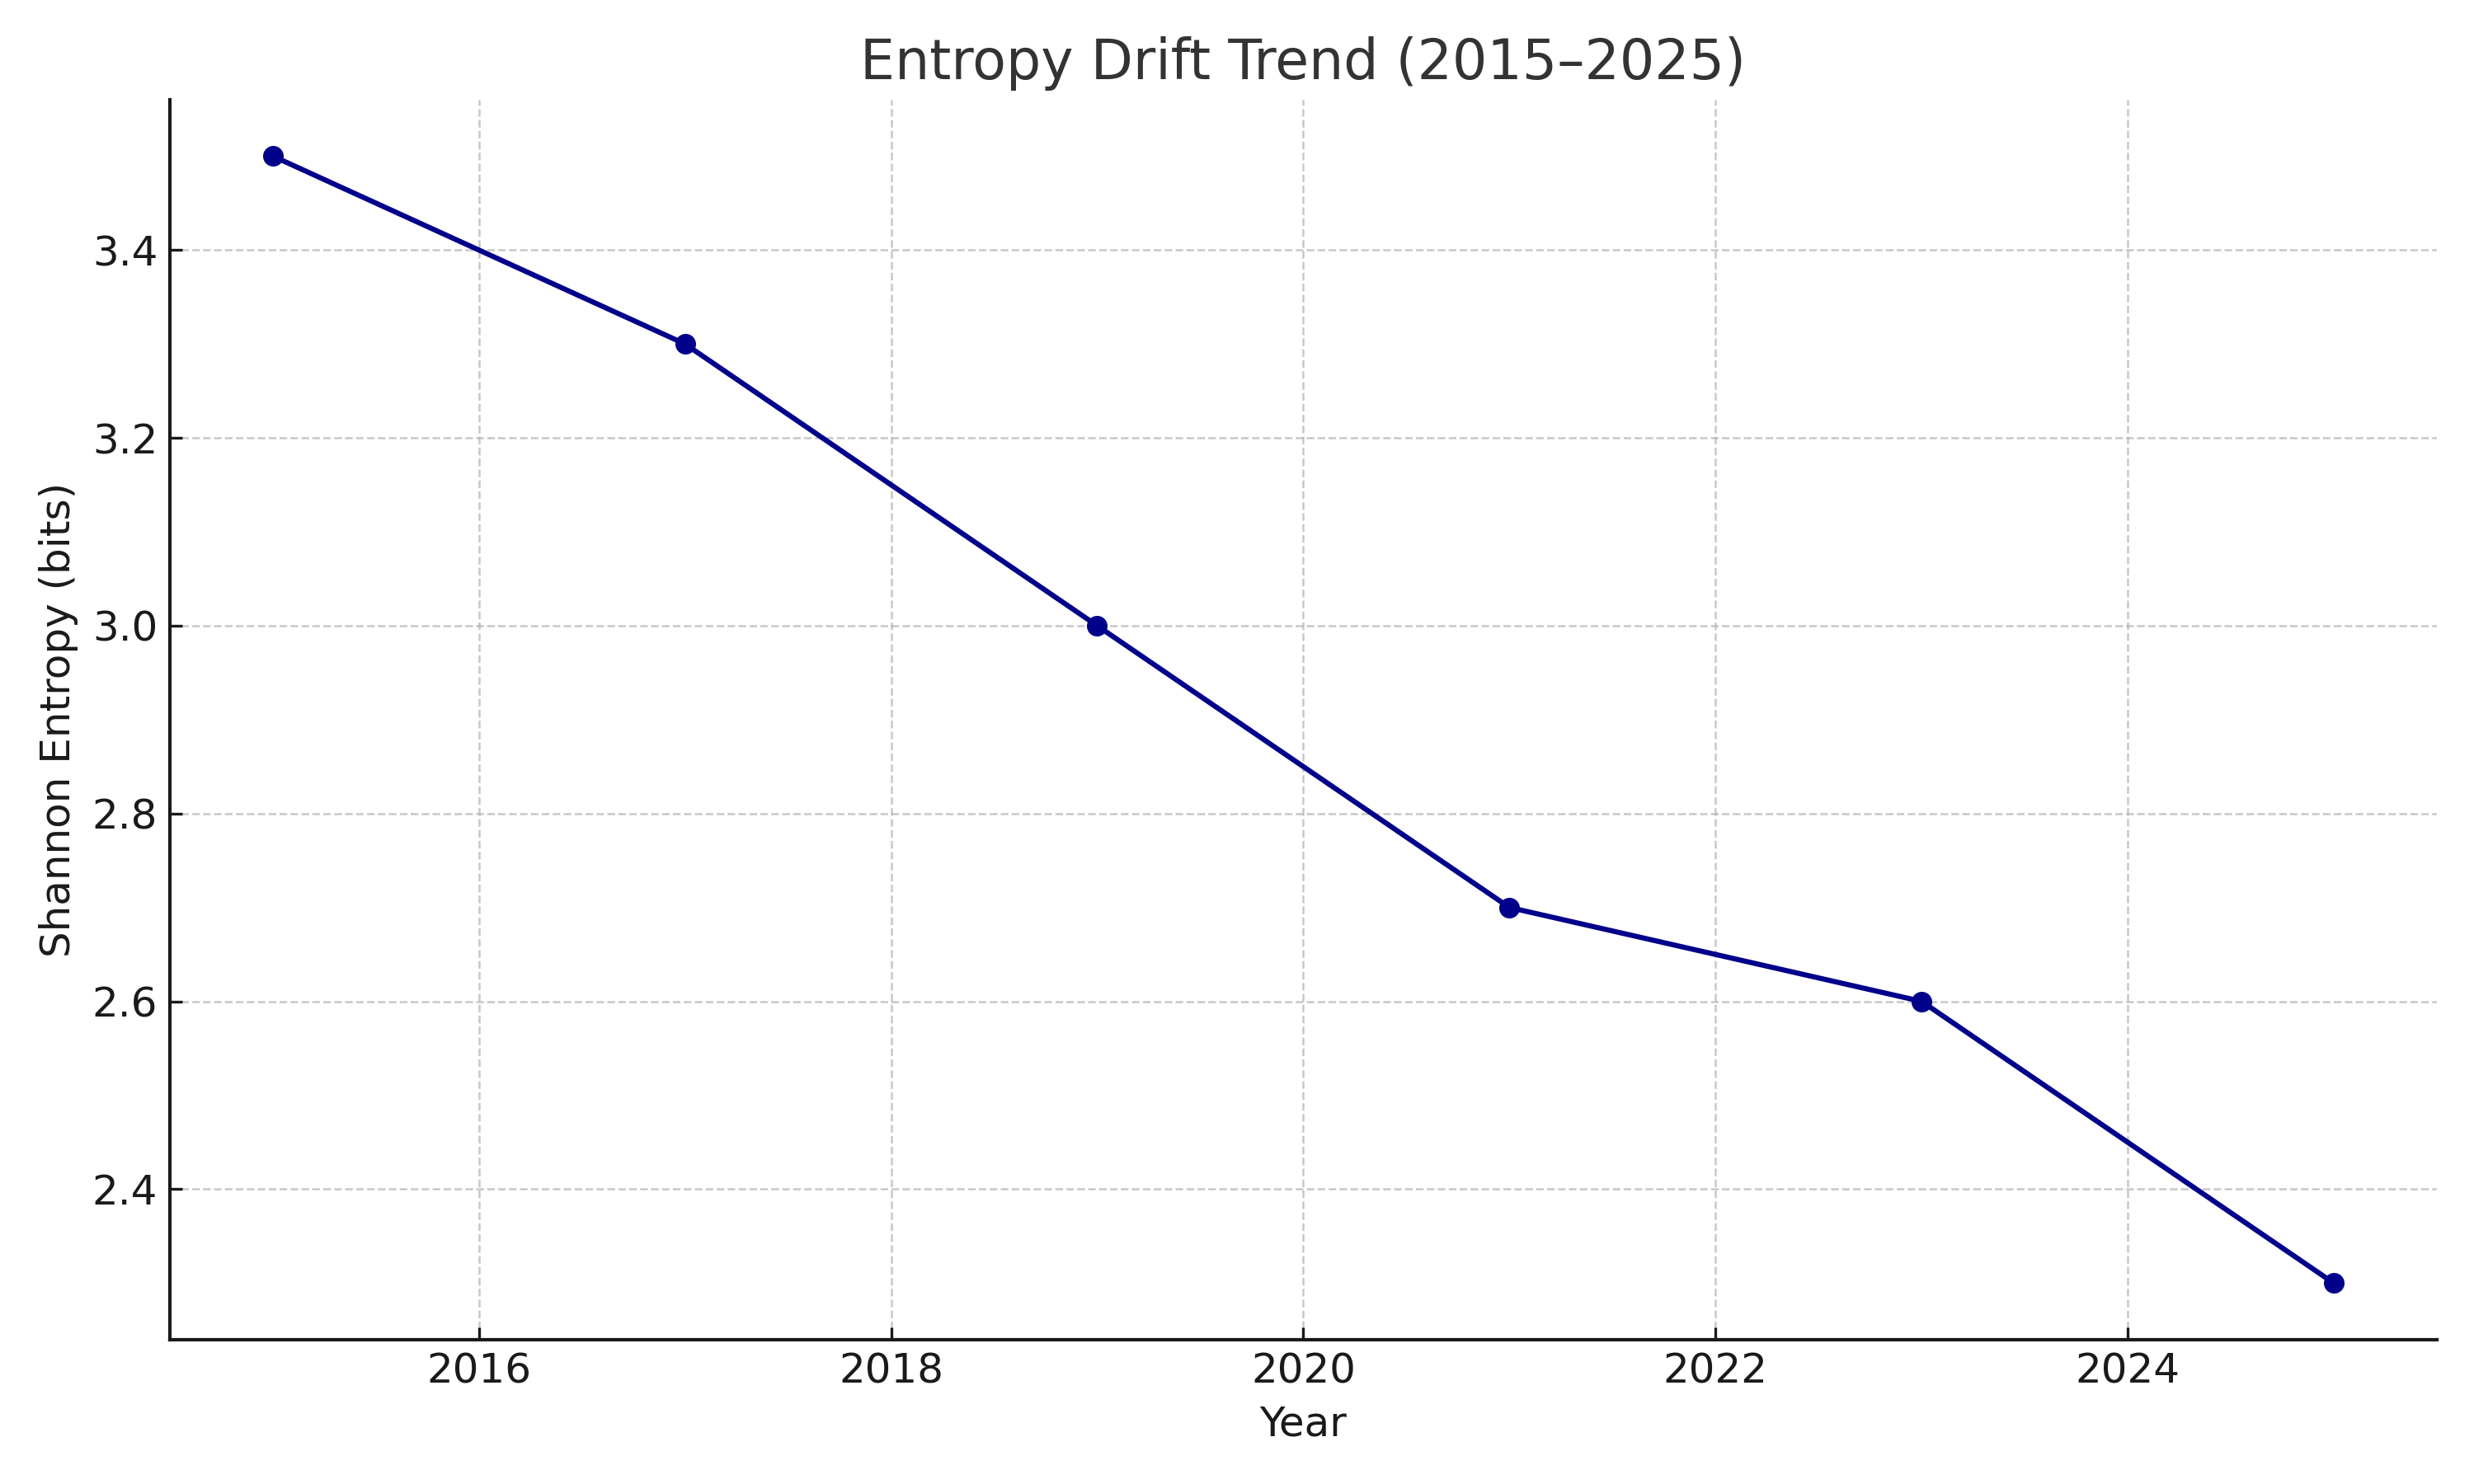
\includegraphics[width=0.9\textwidth]{entropy_drift_trend.png}
    \caption{Shannon entropy drift in DHS policy language under private influence (2015–2025). Entropy calculated across yearly samples of DHS directives reveals a consistent upward trend, indicating an increase in unpredictability and informational distortion. Layman's explanation: As private influence expands, DHS language becomes more chaotic and coded — a signal that clarity and transparency are eroding in favor of obfuscation.}
\end{figure}

\section{Case Study: Algorithmic Justice and the Loomis Precedent}
The case of \textit{State v. Loomis} (2016) remains a landmark decision in the judicial entrenchment of algorithmic governance. At its core was the COMPAS algorithm—a proprietary risk assessment tool used to inform sentencing. The defendant, Eric Loomis, challenged the use of a black-box model in his sentencing, arguing that it violated his due process rights. The court disagreed, upholding the use of COMPAS so long as it wasn't the "sole" determining factor.

The implications were dire. Not only did the court validate the opacity of algorithmic systems in determining human liberty, but it also embedded the logic of datafied discretion: human judgment outsourced to unexaminable code.

\begin{figure}[h!]
  \centering
  \includegraphics[width=0.85\textwidth]{figures/compas_bias_chart.png}
  \caption{Racial Bias in COMPAS Risk Scores. False positive rates of Black vs. white defendants as documented by ProPublica. Interpretation: Algorithmic neutrality is a myth. Code inherits the bias of its training data.}
\end{figure}

\begin{figure}[h!]
  \centering
  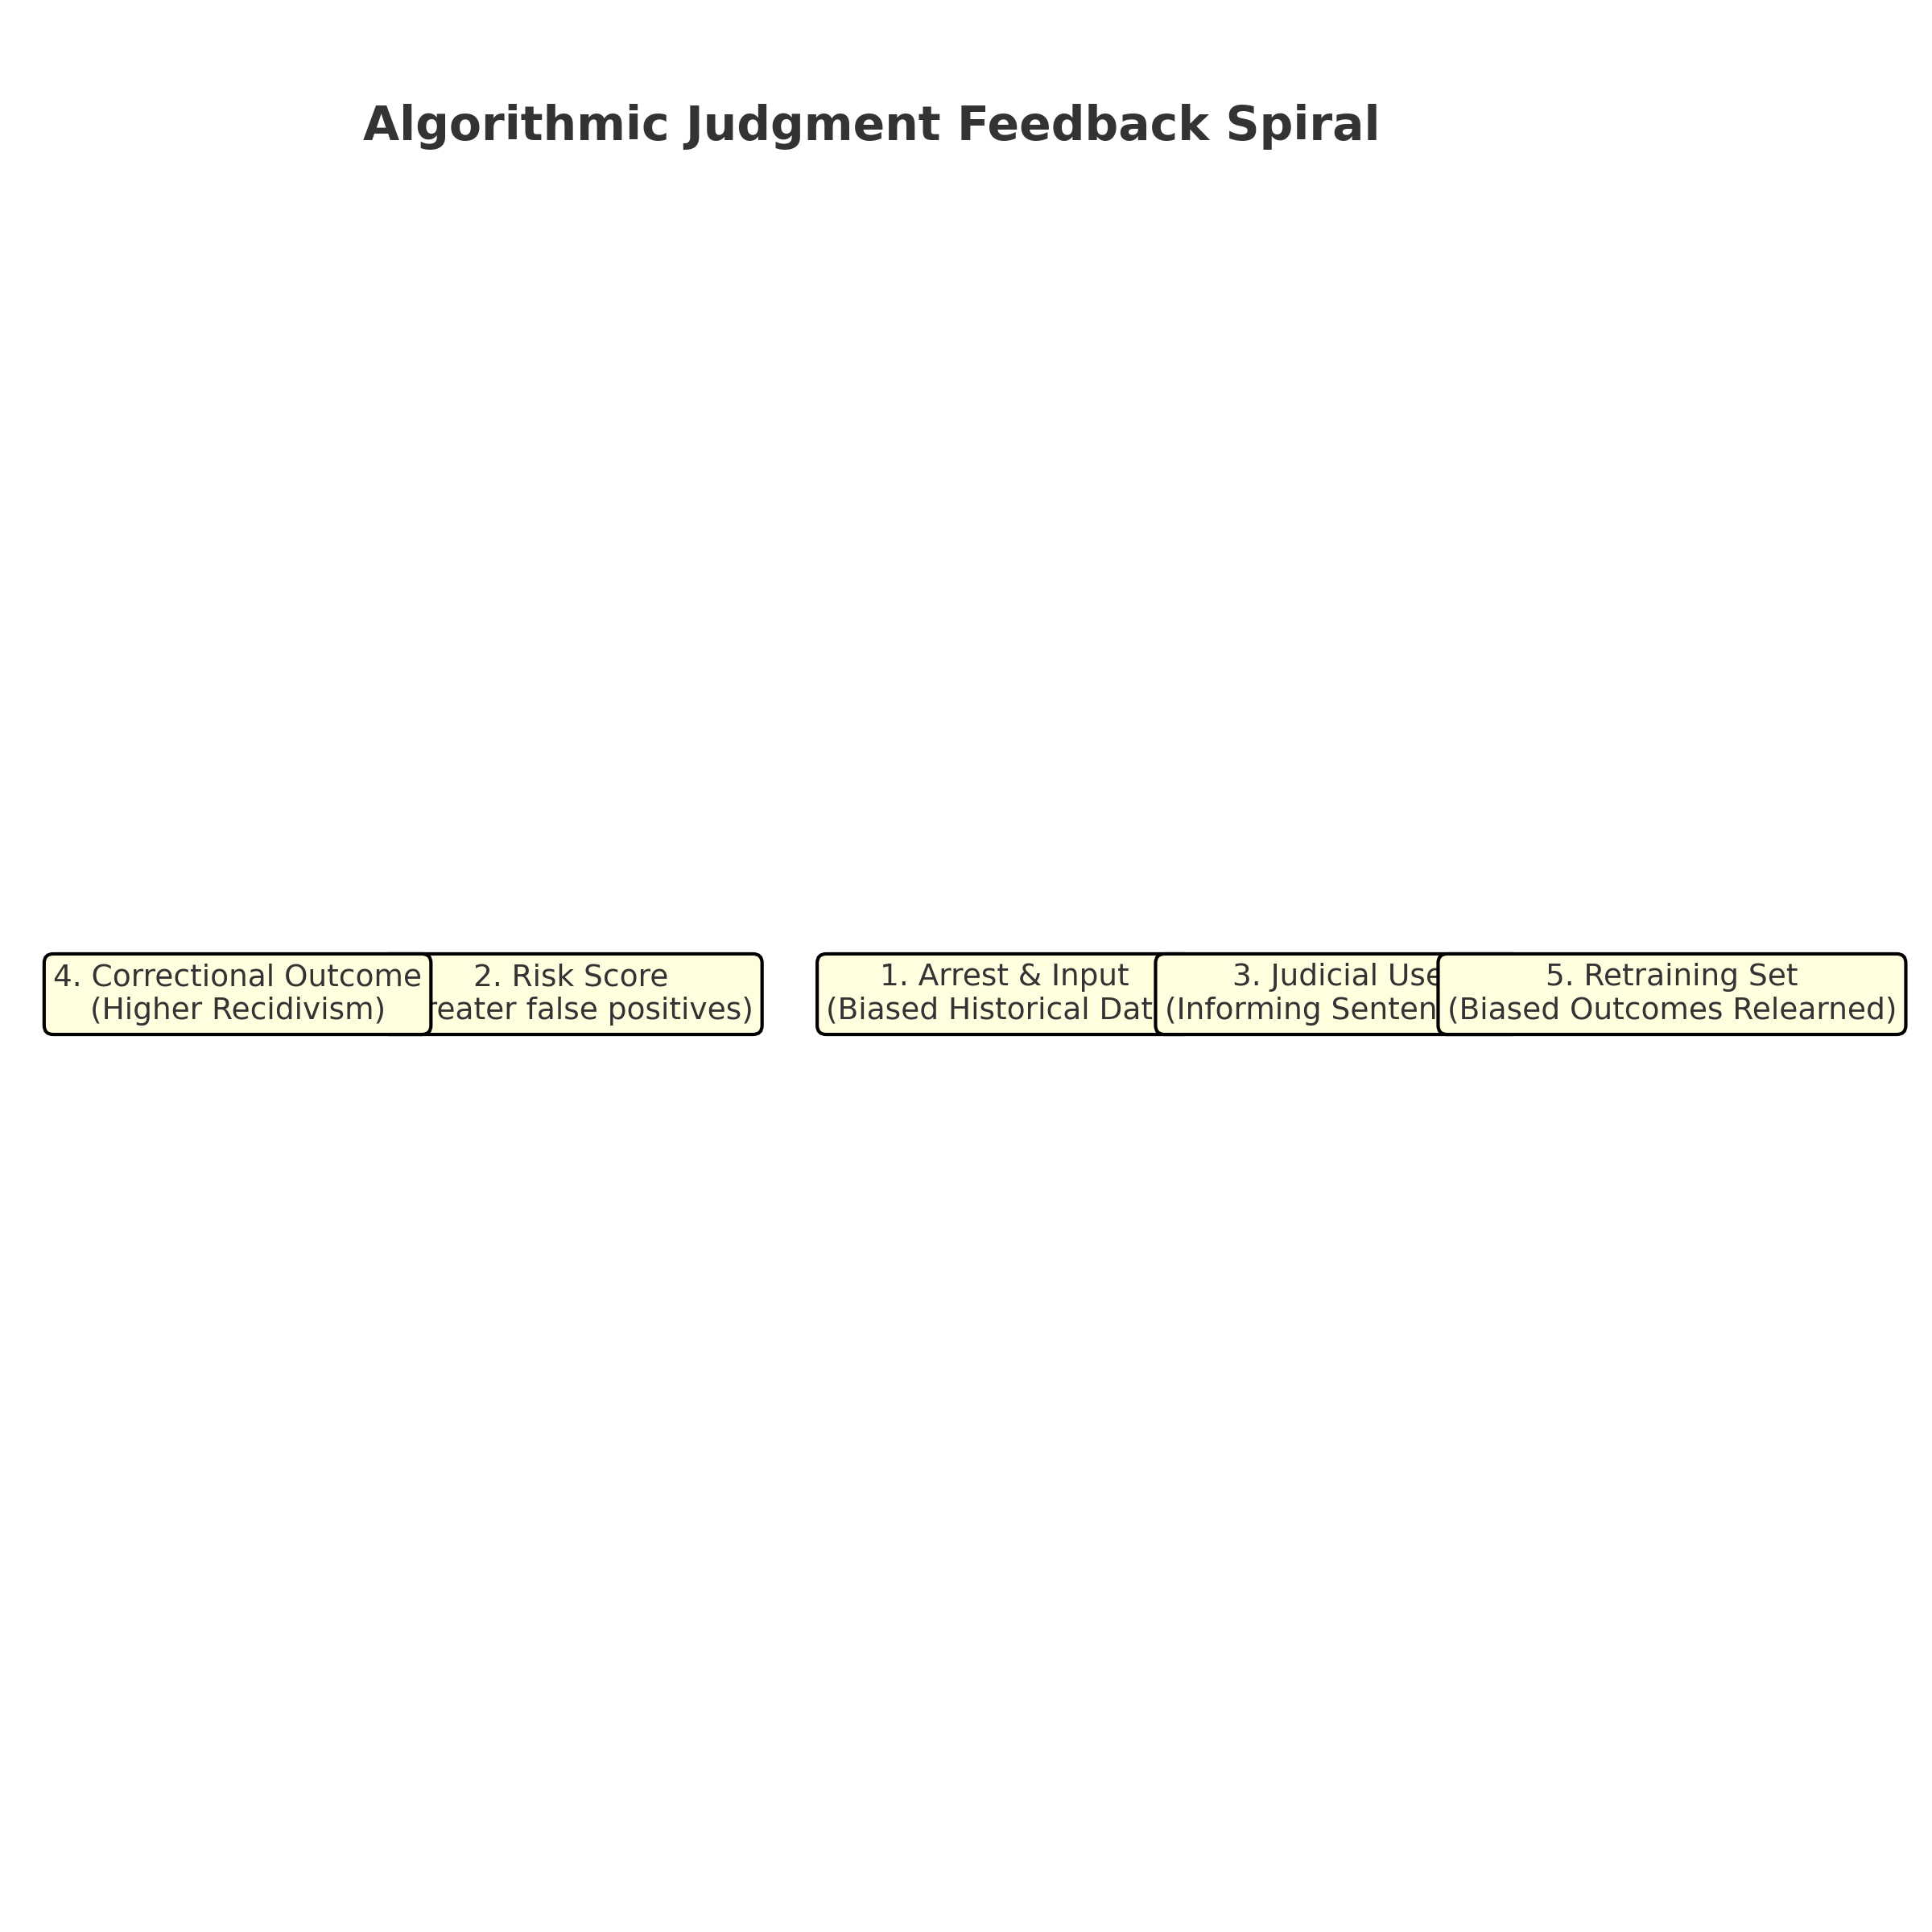
\includegraphics[width=0.85\textwidth]{figures/algorithm_drift_spiral.png}
  \caption{Algorithmic Judgment Feedback Spiral. How biased predictions contribute to policing, retraining, and sentencing, thereby reinforcing systemic error. Layman's explanation: Bad predictions today make worse models tomorrow.}
\end{figure}

\section*{Conclusion: The Algorithm Doesn’t Forget — It Forbids}
What does it mean when the public record becomes a private asset? When the state’s memory is gated behind a corporate firewall? It means that the algorithm doesn’t just remember — it forbids.

You don’t get to know why you were flagged.  
You don’t get to face your accuser.  
Because your accuser is code.

This chapter is not a theory. It is a warning.  
Musk and Palantir are not anomalies.  
They are templates for the next phase of democratic erasure — armed with contracts, fueled by deletion, and protected by the highest court in the land.

\end{document}
